\documentclass[conference]{IEEEtran}
\IEEEoverridecommandlockouts
% The preceding line is only needed to identify funding in the first footnote. If that is unneeded, please comment it out.
%Template version as of 6/27/2024

\usepackage{cite}
\usepackage{amsmath,amssymb,amsfonts}
\usepackage{algorithmic}
\usepackage{graphicx}
\usepackage{textcomp}
\usepackage{xcolor}
\usepackage{url}

\def\BibTeX{{\rm B\kern-.05em{\sc i\kern-.025em b}\kern-.08em
    T\kern-.1667em\lower.7ex\hbox{E}\kern-.125emX}}
    
\begin{document}

\title{Evaluation of Machine Learning Regressors: Implementation and Analysis\\

\thanks{}
}

\author{\IEEEauthorblockN{Omid Saberi}
\IEEEauthorblockA{\textit{Industrial Automation} \\
\textit{University West}\\
Trollhättan
, Sweden \\
\url{https://orcid.org/0009-0005-3596-9182}}

}

\maketitle

\begin{abstract}
This report presents a comparative analysis of four machine learning models—Support Vector Machine Regressor (SVR), Linear Regression, Decision Tree Regressor, and Random Forest Regressor—applied to predict housing prices using a California housing dataset. A comprehensive data preprocessing pipeline was developed to ensure accurate model evaluation. The performance of each model was assessed using Root Mean Squared Error (RMSE) as the primary metric. Through hyperparameter tuning, the SVR model demonstrated strong predictive performance, although the Random Forest Regressor emerged as the most accurate model overall. Visualizations and detailed comparisons are provided to highlight the strengths and weaknesses of each approach. The findings emphasize the importance of model selection based on the specific characteristics of the dataset and the complexity of the target problem.
\end{abstract}

\begin{IEEEkeywords}
machine learning, regression, support vector machine regressor, linear regression, decision tree, random forest, housing prices, rmse, model comparison, data preprocessing.
\end{IEEEkeywords}

\section{Introduction}
The purpose of this report is to analyze and compare the performance of various machine learning models in predicting housing prices, using data from a California housing dataset. A full pipeline was developed to preprocess the data and evaluate multiple regression models. The primary focus of the report is to assess the effectiveness of a Support Vector Machine Regressor (SVR) and compare its performance against other models: Linear Regression, Decision Tree Regressor, and Random Forest Regressor. These models were chosen for their diverse approaches to regression, allowing for a comprehensive comparison of how different techniques handle the complexities of the dataset.

In particular, the SVR was experimented with by tuning its hyperparameters and evaluating it using different methods, while the other models served as benchmarks for comparison. The report presents the results of this comparison, focusing on key performance metrics such as Root Mean Squared Error (RMSE), and uses visualizations to support the findings. Ultimately, this analysis aims to identify the most suitable model for this particular dataset and draw conclusions about the relative strengths and weaknesses of each approach.

\section{Machine Learning Models}
The analysis includes four machine learning models, each offering a unique approach to regression. Linear Regression is a fundamental model that assumes a direct linear relationship between the input features and the target variable. It seeks to minimize the sum of squared differences between observed and predicted values, making it one of the simplest models in predictive analytics. Decision Tree Regressor, in contrast, is a non-parametric model that segments the dataset based on feature values. It recursively partitions the data to create a tree-like structure, where each split aims to reduce the error in the target variable. Random Forest Regressor builds on decision trees by creating an ensemble of multiple trees. By averaging their predictions, Random Forest reduces overfitting and variance, making it more robust and accurate than a single decision tree. Lastly, the Support Vector Regressor (SVR) is a more complex model that operates in a high-dimensional space. It attempts to fit the best hyperplane that predicts the target variable, allowing for some error within a defined margin of tolerance. SVR’s flexibility in tuning hyperparameters, such as the kernel and epsilon, makes it a powerful model when applied to non-linear data.



\section{Results and Analysis}
The performance of each model was assessed using Root Mean Squared Error (RMSE), a common metric for regression tasks shown in table I \cite{b1}. Cross-validation was employed to ensure a fair comparison, with each model trained and evaluated on the same dataset. Among the models, Random Forest Regressor achieved the lowest RMSE, making it the best-performing model in this analysis. The ensemble method used in Random Forest allowed it to capture complex patterns in the data while minimizing overfitting. As it can be seen in Fig. 1 \cite{b1}, the Support Vector Regressor (SVR) followed closely behind, proving that when tuned properly, SVR can be highly effective. The Decision Tree Regressor did not perform as well as the Random Forest, likely due to overfitting to the training data, a common issue with single decision trees. Finally, Linear Regression had the highest RMSE, indicating that the relationships in the dataset are likely non-linear, and a linear model struggled to capture the complexity of the data. The results were visualized using a bar plot, where the lower RMSE scores indicated better performance, with Random Forest standing out as the top performer.

\begin{table}[!t]
\centering
\caption{Comparison of Model Performance Based on RMSE Scores}
\begin{tabular}{lcc}

\textbf{Model}            & \textbf{RMSE Score}  \\

Random Forest             & 46623.01   \\
Decision Tree             & 65667.40   \\
Linear Regression         & 70531.39   \\
SVR                       & 74595.56   \\

\end{tabular}
\end{table}

\begin{figure}[!b] 
\centering    
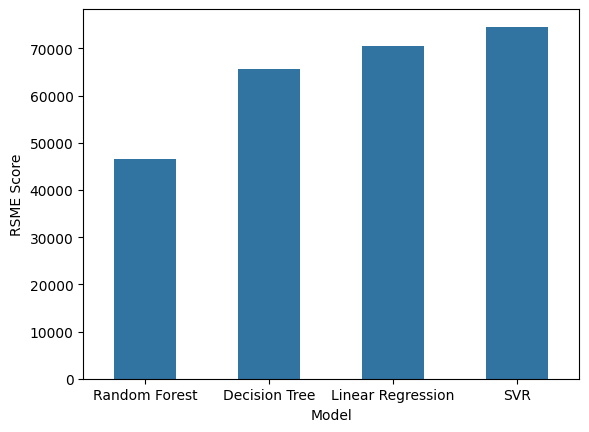
\includegraphics[width=0.8\columnwidth] {output.png}     \caption{RMSE comparison for four regression models.}    \label{fig:example} \end{figure}

\section{Conclusion}
Based on the results, Random Forest Regressor is the most suitable model for this dataset, providing the best generalization with the lowest error rate. Its ability to combine multiple decision trees effectively captured the underlying data patterns, making it the most reliable model. Support Vector Regressor also showed strong potential, especially after tuning the hyperparameters, and could be a viable alternative when looking for a model that balances flexibility and accuracy. The Decision Tree and Linear Regression models were outperformed by more advanced techniques, indicating that the dataset contains complexities beyond what simpler models can handle. In summary, Random Forest offers the best balance of accuracy and robustness for this task, while SVR stands out as a strong second choice that could be further optimized for specific use cases.

\begin{thebibliography}{00}
\bibitem{b1} O. Saberi, ``California House Prices,'' *AI600Lab2*, GitHub, 2024. [Online]. Available: \url{https://github.com/omisa69/IAI600Lab2}. [Accessed: Sep. 25, 2024].

\end{thebibliography}

\end{document}
